\subsection{1.2.1.5 Properties}
\begin{frame}{Definitions}
We call $(V,\mathbb{T})$ 
\begin{itemize}
    \item \textbf{Well-posed} if each $T_\sigma\in\mathbb{T}$ has a unique fixed point in $V$
    \item \textbf{Regular} if $V_G=V$, that is all $v\in V$ has a greedy policy
    \item \textbf{Bounded above}, there exists $u\in V$ such that $T_\sigma u \precsim u$ for all $T_\sigma\in \mathbb{T}$
    \item \textbf{Downward stable/Upward stable/Order stable/Strongly Order stable/ Order continuous} if each $T_\sigma\in\mathbb{T}$ is downward stable/$\cdots$
\end{itemize}

\end{frame}
\begin{frame}{Definitions}
\begin{definition}
    Let $V$ be a poset and $S$ be a self-map on $V$. In this setting, we call $S$
    \begin{itemize}
        \item \textbf{upward stable} on $V$ if $S$ has a unique fixed point $\bar v\in V$, and, in addition, if $v\in V, v\precsim Sv$, then $v\precsim \bar v$
        \item \textbf{downward stable} on $V$ if $S$ has a unique fixed point $\bar v\in V$, and, in addition, if $v\in V, Sv\precsim v$, then $\bar v\precsim v$
        \item \textbf{order stable} if $S$ is both upward stable and downward stable
    \end{itemize}
\end{definition}
    
\end{frame}

\begin{frame}{Definitions}
\begin{definition}
Let $V$ be a poset and $S$ be a self-map on $V$. In this setting, we call $S$
\begin{itemize}
    \item \textbf{Strongly upward stable} on $V$ if $S$ has a unique fixed point $\bar v$, and, if $v\in V, v\precsim Sv$, then $S^nv\uparrow \bar v$
    \item \textbf{Strongly downward stable} on $V$ if $S$ has a unique fixed point $\bar v$, and, if $v\in V, Sv\precsim v$, then $S^nv\downarrow \bar v$
    \item \textbf{Strongly order stable} on $V$ if $S$ is both strongly upward stable and strongly downward stable.
\end{itemize}
\end{definition}
\end{frame}
\begin{frame}{Order continuity}

    \begin{definition}
    Let $V, W$ be posets. We call $S: V\to W$ \textbf{order continuous} if 
    $$
    v_n\uparrow v \implies Sv_n\uparrow Sv
    $$
    In other words, if $(v_n)\subset V$ with $v_n\uparrow v\in V$, then $\bigvee_n S v_n = Sv\in W$.
     \end{definition}
     \begin{lemma}
         Every order continuous map is order preserving.
     \end{lemma}
     \begin{proof}
         Apply to this sequence $\{v,v',v',\cdots\}$, where $v\precsim v'$
     \end{proof}
\end{frame}
\begin{frame}{Importance of Order continuity}
\textbf{Remark}: With only order preserving and order stability, we \textbf{cannot guarantee} an iterating bound monotone sequence converge to the unique fixed point.
    
\end{frame}
\begin{frame}{Example: without continuity}
\begin{figure}
    \centering
    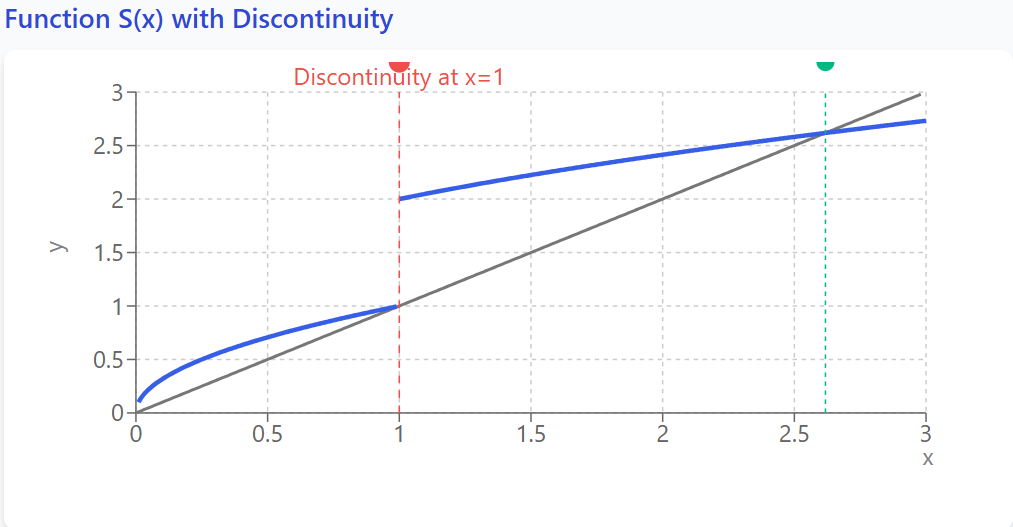
\includegraphics[width=1\linewidth]{Dynamic Programming/DP2/Chapter 1/Section 1.2/figure/discontinuous.png}
\end{figure}
    
\end{frame}

\begin{frame}{Convergence}
\begin{figure}
    \centering
    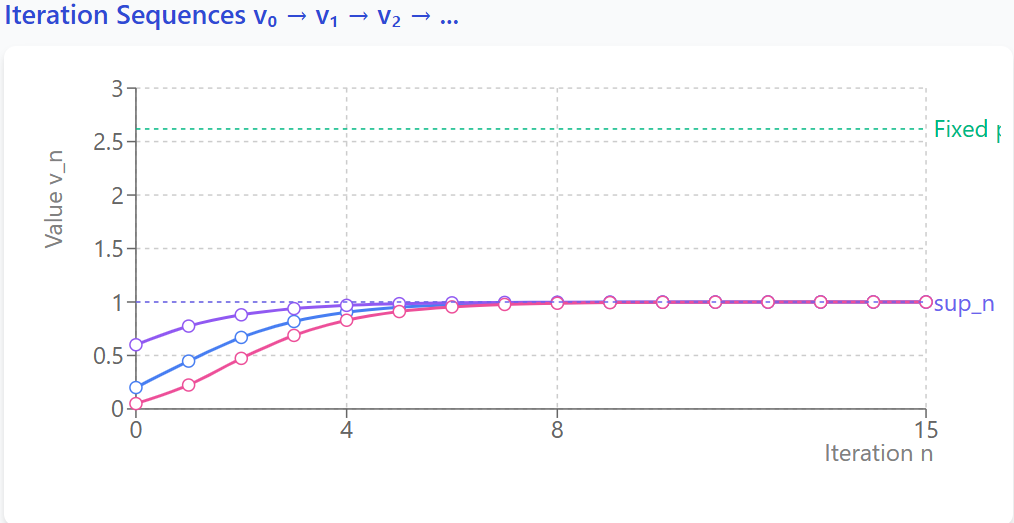
\includegraphics[width=1\linewidth]{Dynamic Programming/DP2/Chapter 1/Section 1.2/figure/convergence.png}
\end{figure}
\end{frame}

\begin{frame}{Order Completeness}
\begin{definition}
    A nonempty poset $V$ is called
    \begin{itemize}
        \item a \textbf{lattice} if every finite subset of $V$ has both a supremum and an infimum in $V$
        \item a \textbf{complete lattice} if every subset of $V$ has a supremum and an infimum in $V$
        \item \textbf{chain complete} if every chain in $V$ has a supremum and an infimum in $V$
        \item \textbf{$\sigma$-chain complete} is every at most countable chain in $V$ has a supremum and an infimum in $V$
    \end{itemize}
\end{definition}
\textbf{Remark:} Here  `finite' means nonempty finite, `at most countable' means empty, finite, or countable. 
    
\end{frame}

\begin{frame}{Chain complete poset is order bounded}

\begin{lemma}
    Let $V$ be any poset. We have
    \begin{itemize}
        \item $b:= \bigvee \emptyset$ exists in $V$ if and only if $V$ has a least element and that least element is $b$
        \item $u:= \bigwedge \emptyset$ exists in $V$ is and only if $V$ has a greatest element and that greatest element is $u$.
    \end{itemize}
\end{lemma}
    \begin{proof}
        Suppose $b=\bigvee\emptyset$ exists in $V$. By definition of empty set, we know that every subset of $V$ is an upper bound of $\emptyset$. In other words, every element of $V$ is in the upper bound of $\emptyset$. Hence, the least upper bound of the emptyset is the least element of $V$.\\
        \\
        Suppose $V$ has a least element and that least element is $b$. Following the above logic, the least upper bound of the emptyset should be the least element of $V$. Given its existence, we know that $b=\bigvee\emptyset$.
    \end{proof}
\end{frame}

\begin{frame}{Chain complete poset is order bounded}
\begin{lemma}
    d
\end{lemma}
    
\end{frame}
